\cotefile{161-3}
\scanpage{22}
et soit $F\xrightarrow{f}G$ dans $\widehat C$, bicouvrant, prouvons que
$\widehat u_{\unsure{\bullet|0}}(F)\xrightarrow{\widehat u_{\bullet}(f)}\widehat u_{\bullet}(G)$ est \deleted{bicouvrant} un isom. On a .....

\[
\deleted{\unsure{F}\mathop{\longrightarrow}_{\unsure{C/X}} \unsure{X}\longrightarrow}
\]
% archive sheet number: 21

\scanpage{24}
\uline{Espaces essentiels et ensembles ordonnés}

$X$ un ensemble

a) $\unsure{\tau|\mathcal T}(X)$ l'ens des topologies sur $X$

$\underline\omega(X)$ \rule{2.6em}{0.35pt} préordres sur $X$

\[
\deleted{\unsure{\alpha_X}}\quad \tau(X)\xrightarrow{\alpha_X}\underline\omega(X)
\]

à $T\in\tau(X)$ est associée la relation $\alpha_X(T)$

\[
y\leq_T x\mathrel{\mathop{\Longleftrightarrow}^{(\text{déf})}}x\in\overline{\{y\}}
\]

\[
\deleted{\unsure{\beta_X}}\quad\tau(X)\xleftarrow{\beta_X}\underline\omega(X)
\]

à la relation $\omega$ $({\leq}_{\omega})$ est associée $T$

\[
\begin{aligned}
&\deleted{\unsure{\{U\subset X\}|\mathrm{Fer}}}\\[-2pt]
\mathrm{Ouv}(T)&=\{\unsure{U|X}\subset X\mid(x\in U,\,y\leq_{\omega}x)\Rightarrow y\in U\}\\
&=\text{réunions quelconques d'ensembles}\\
&\phantom{=}\text{de la forme }\ O_x=(\unsure{]\leftarrow,x]})=\{y\in X\mid y\leq_{\omega} x\}
\end{aligned}
\]

\[
\mathrm{Fer}(T)=\{Z\subset X\mid(x\in Z,\,y\unsure{\geq|\leq}_{\omega}x)\Rightarrow y\in Z\}
\]

$\alpha$ et $\beta$ fonctoriels en l'ensemble $X$
(pour images inverses de top. resp. de relations d'ordre)

b) Soit $f:X\longrightarrow X'$ une application, \deleted{$X$ muni de $(T,\omega)$, $X'$ de $( $}
si $X,X'$ sont des espaces top. et si $f$ est \deleted{croissante}\inserted{continue}, $f$ est croissante
si $X,X'$ sont préordonnés et si $f$ est croissante, $f$ est continue

$\unsure{\therefore|\text{c)}}$ Deux foncteurs

\diagram{\begin{tikzcd}[ampersand replacement=\&]
\deleted{\unsure{\alpha}}\quad(\mathrm{Esp}) \arrow[r,shift right,"\alpha"'] \& (\mathrm{Préor}) \arrow[l,shift right,"\beta"']
\end{tikzcd}}

c) \deleted{\unsure{Définition de}}
Soit $T\in\tau(X)$, montrer que \unsure{pour} tout ouvert de $X$ est stable par générisation
(\deleted{\unsure{ou|resp.}} tout fermé de $X$ stable par spécialisation), i.e. ouvert pour $\dot\alpha_X(T)$, i.e.

\[
T\leq\beta_X\alpha_X(T)\deleted{\unsure{\leq}}
\]

i.e on a une application continue

\[
\beta\alpha(X)\longrightarrow X
\]

dont l'application sous-jacente est l'identité, d'où une transfo fonctorielle en $X$

\[
\beta\alpha\xrightarrow{\rho}\mathrm{id}_{(\mathrm{Esp})}
\]

Soit $\omega\in\underline\omega(X)$, \deleted{\unsure{munissons $X$ de}} $T=\beta_X(\omega)$, alors $x\in\overline{\{y\}}$ sss
le plus petit ouvert $O_x$ contenant $x$ contient $y$, i.e. sss $y\geq x$, donc on trouve

\[
\alpha_X\beta_X(\omega)=\omega
\]

i.e. on a un isomorphisme

\[
X\xrightarrow{\overset{\sigma}{\sim}}\alpha\beta(X)
\]

tel que l'application ensembliste sous-jacente soit l'identité, d'où

\[
\mathrm{id}_{(\mathrm{Préor})}\xrightarrow{\overset{\sigma}{\sim}}\alpha\beta
\]

d) Montrer que $\rho$ et $\sigma$ sont des morphismes d'adjonction, associés,
établissant pour

\[
X\in\mathrm{Ob}(\mathrm{Esp})\qquad I\in\mathrm{Ob}(\mathrm{Préor})
\]
% archive sheet number: 23

\scanpage{25}
une bijection

\[
\operatorname{Hom}_{\mathrm{Esp}}(\beta I,X)\simeq\operatorname{Hom}_{\mathrm{Préord}}(I,\alpha X)\tag*{$(*)$}
\]

% slanted
\margin{\uline{Cor} le foncteur $\alpha$ $(\mathrm{Esp})\to(\mathrm{Préor})$ commute aux $\varprojlim$ le foncteur $\beta$ aux $\varinjlim$. Mais de plus $\beta$ est \uline{exact à gauche} i.e. sur $X\times Y$ la top. associée au préordre produit est le produit des topologies (Mais $\beta$ ne commute pas aux produits quelconques, un \deleted{foncteur} produit d'espaces topologiques essentiels \unsure{discrets} dont les pts sont essentiels n'est pas néc. essentiel. Ex. produit infini d'espaces top. \uline{discrets}.}

\unsure{$*$ exprime|En effet}: une application

\[
I\xrightarrow{f}X
\]

est croissante sss elle est continue (\unsure{$[$}$X$ étant muni de la
relation d'ordre $\alpha_X(T_X)$, $I$ de la topologie $\beta_I(\omega_I)$).
En effet, si $f$ est continue, on sait qu'elle est croissante pour les
\deleted{topologies}\inserted{ordres} associés aux topologies, or ce sont l'ordre de départ de $I$, et $\uline{\alpha_X(T_X)}$.
Et si $f$ est croissante, \deleted{\unsure{soit ouvert dans $X$}} l'image inverse d'une partie de $X$
ouverte pour $\beta_X\alpha_X(T_X)$ est ouverte dans $I$, mais toute partie
\deleted{\unsure{de $I$}} de $X$ \inserted{ouv\textsuperscript{te}} l'est pour $\beta_X\alpha_{\unsure{\alpha|X}}(T_X)$, donc on a gagné.

e) \uline{Corollaire} Le foncteur

\[
\beta:(\mathrm{Préord})\longrightarrow(\mathrm{Esp})
\]

est pleinement fidèle. Son image essentielle est formée des
espaces $(X,T_X)$ pour lesquels $T_X\in\beta_X(\underline\omega(X))$ ; ce sont aussi
les espaces topologiques pour lesquels tout point $x\in X$ a un
plus petit voisinage ouvert $O_x$. [C'est évidemment nécessaire ;
\deleted{\unsure{et}} pour prouver que c'est suffisant, il faut pr. que

\[
O_x=\{y\in X\mid y\leq_T x\}.
\]

Mais \deleted{\unsure{évident, $O_x$ étant}} \deleted{pour prouver $\subset$, noter que si $y\in O_x$, \unsure{on a} $O_y$}
$x\in\overline{\{y\}}$ signifie évidemt ($O_x$ étant le plus petit \deleted{ouvert}\inserted{voisinage} de $x$)
que $O_x\ni y$, OK.

\margin{NB les topologies obtenues sont aussi celles pour lesquelles toute intersection d'ouverts est ouverte [NB Ce n'est pas stable par passage à l'espace sobre associé ....]}

f) Soit \deleted{\unsure{un}} $X,T$, alors $X$ est présobre $(\overline{\{x\}}=\overline{\{y\}}\ \Rightarrow\ x=y)$
\deleted{\unsure{g)}} sss \deleted{\unsure{le}} préordre $\omega(T)$ est un \uline{ordre}. \deleted{\unsure{$X$}},

\deleted{g) Soit $X$ muni d'un préordre, d'où topologie associée. Désignons par $\underline X$ la catégorie associée à $X$ ordonné ($\operatorname{Hom}(x,y)=\begin{cases}\varnothing&\text{si }\deleted{\unsure{y}}\,x\nleq y\\\{e\}&\text{si }\deleted{\unsure{x}}\,x\leq y\end{cases}$ i.e. $\operatorname{Hom}(x,y)\ne\varnothing$ sss $O_y\supset O_x$) Montrer que le \deleted{foncteur}}

\deleted{$F\longmapsto(x\mapsto F(O_x))$ de $\operatorname{Top}(X)$ dans $\widehat{\underline X}$ est une équivalence de cat.}

\[
\deleted{\operatorname{Top}(X)\simeq\widehat{\underline X}}
\]

\deleted{On identifie les $x\in X$ à des sous-objets de $e_{\widehat{\underline X}}$, et les cribles de $X$ (i.e. \inserted{des ouverts de $\widetilde X$} ouverts de $X$) à des s-objets de $e_{\widehat{\underline X}}$, i.e.}
% archive sheet number: 24

\scanpage{26}
g) $X$ muni d'une topologie $T$ déduite d'un préordre $\omega$ [donc les ouverts
sont les réunions d'ens de la forme $O_x$, $x\in X$]. $X$ est irréductible
sss deux ouverts non vides ont une intersection non vide, i.e. pour
$x,y\in X$, $O_x\cap\unsure{U_y|O_y}\ne\varnothing$ i.e. $\forall x,y\in X$, $\exists z\in X$ avec $z\leq x,\ z\leq y$,
i.e. $X$ est \uline{cofiltrant}. En conclure que les fermés irréductibles
de $X$ sont les parties $Y$ de $X$ telles que

\[
\begin{aligned}
&\text{a)}\quad y\in Y,\ \inserted{y'\in X,}\ y'\geq y\Rightarrow y'\in Y\qquad(Y\text{ fermé})\\
&\text{b)}\quad\forall x,y\in Y,\ \exists z\in Y,\ \text{tel que }\ z\leq x,\ z\leq y.
\end{aligned}
\]

h) $X$ comme dans g), $\underline X$ la catégorie associée à la relation de \inserted{pré}ordre
$\operatorname{card}\operatorname{Hom}_{\underline X}(x,y)\leq1$, $\deleted{\unsure{\mathrm{Hom}}}\operatorname{Hom}_{X}(x,y)\ne\varnothing\Leftrightarrow x\leq y\Longleftrightarrow y\in\overline{\{x\}}$ ---
Considérons le foncteur $\operatorname{Top}(X)\mathbin{\unsure{-|\to}}\widehat{\underline X}$, $F\longmapsto(x\longmapsto F(O_x))$.

Prouver que ce foncteur est une équivalence

\[
\operatorname{Top}(X)\mathrel{\overset{\sim}{\simeq}}\widehat{\underline X}
\]

Désormais on identifie [$\deleted{\unsure{X|\text{si}}}$ $X$ présobre i.e. \uline{ordonné}] $X$ à un
ensemble de sous-objets de l'objet final de $\widehat{\underline X}=\operatorname{Top}(X)$
[\deleted{\unsure{c.à.d|cribles}} d'ouverts du topos), et de $=$ pour les ouverts de $X$,
identifiés à des s-objets de $e_{\widehat{\underline X}}$ donc à des ouverts du topos.

Interpréter

\[
\underline{\operatorname{Points}}(\widehat{\underline X})\simeq\operatorname{Pro}(\underline X)
\]

en identifiant les pro-objets de $\underline X$ \inserted{(mod iso)} aux sous-ensembles
ordonnés $Y$ de $X$ satisfaisant les conditions a) b) de g),
\deleted{\unsure{avec|et}} la structure de catégorie provenant de la relation
d'ordre entre parties de $X$ \uline{opposée} de la relation d'inclusion.
Soit \deleted{\unsure{Privé de|$\operatorname{Pro}(X)$}}\inserted{$\widetilde X$} nouvel ens. ordonné ainsi construit. L'application
$x\longmapsto\overline{\{x\}}=\{y\in X\mid y\geq x\}$ est une application $X\mathbin{\unsure{-|\to}}\widetilde X$, qui
s'identifie à l'application can. de $X$ dans l'espace sobre
associé, \uline{ou} à $\underline X\longrightarrow\operatorname{Pro}(\underline X)$ (foncteur canonique).

i) \uline{Conditions équivalentes} $\alpha)$ $X\longrightarrow\widetilde X$ surjective
$\beta)$ Toute partie fermée cofiltrante de $X$ a un plus petit élément.
% archive sheet number: 25

\scanpage{27}
$\gamma)$ \deleted{$T_0$} $X$ (pour sa relation d'ordre) est artinien, i.e. tout
\deleted{famille}\inserted{suite} décroissante d'éléments de $X$ est \unsure{station.}

$\delta)$ $\widetilde X$ est essentiel (i.e. chaque pt de $X$ est essentiel)

\margin{en fait, $\operatorname{Im}(X\to\widehat X)$ est l'ens des pts ess. de $\widetilde X$ !}

j) Soit $E$ un topos. Conditions équivalentes

$\alpha)$ $E$ \deleted{\unsure{isom.|n'est}}\inserted{équiv.} à un $\operatorname{Top}(X)$ \uline{et} à un $\widehat C$

$\beta)$ $E$ équiv. à $\operatorname{Top}(X)$, $X$ espace essentiel

$\gamma)$ $E$ équ. à $\widehat I$, $I$ ens. ordonné

$\delta)$ $E$ engendré par les sous-objets de l'objet final, et
a suff. de pts essentiels

[\deleted{\unsure{On}}\unsure{On} dit alors que $E$ ``est'' un espace top. essentiel.]

Prouver que si $C$ est une catégorie, $\widehat C$ satisfait aux conditions
précédentes sss $C$ est préordonnée.

Prouver que si $X$ est un espace top, $\operatorname{Top}(X)$ satisfait aux
conditions précédentes sss l'ens des $x\in X$ qui sont
essentiels est très dense.

\deleted{\unsure{k) Soit $X$}}
On a des équivalences de 2-catégories

\[
(\text{topos spatiaux essentiels})\mathrel{\overset{\approx}{\simeq}}
\deleted{\text{ens. ordonnés}}\inserted{(\mathrm{Préord})}
\mathrel{\overset{\approx}{\simeq}}(\mathrm{Esp.ess.})
\]

[NB. Si $X$ est \unsure{esp.|ess.} on le récupère à partir de $E=\operatorname{Top}(X)$ comme $\underline{\mathrm{Points}}(\unsure{E_{\mathrm p}|E})$]
% archive sheet number: 26

\scanpage{29}
$\unsure{\gamma}$ commute aux Inf finis ?

\[
\begin{aligned}
\deleted{\unsure{\alpha(}}\qquad \unsure{\gamma|\alpha}(X\times Y)&=\alpha(X)\beta(Y)=1_O\\
\gamma(W\cap W')&=\operatorname*{Sup}_{U\times V\subset W\cap W'}\alpha(U)\cap\beta(\unsure{W|V})
=\operatorname*{Sup}_{\substack{U\times V\subset W\\ U'\times V'\subset W'}}
 \underbrace{\alpha(U\cap U')\cap\beta(V\cap V')}_{\underbrace{\alpha(U)\beta(V)}\quad\underbrace{\alpha(U')\beta(V')}}\\
&=\operatorname*{Sup}_{U\times V\subset W}\alpha(U)\beta(V)\ \wedge\operatorname*{Sup}_{U'\times V'\subset W'}\alpha(U')\beta(V')\\
&=\unsure{\gamma|\mathcal R}(W)\cap\gamma(W')
\end{aligned}
\]

\figure{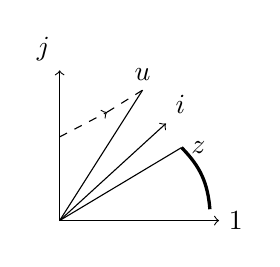
\begin{tikzpicture}[scale=.9]
\draw[->] (0,0)--(2.25,0) node[right] {$1$};
\draw[->] (0,0)--(0,2.12) node[above left] {$j$};
\draw[->] (0,0)--(1.50,1.37) node[above right] {$i$};
\draw (0,0)--(1.72,1.03) node[right] {$z$};
\draw[very thick] (1.72,1.03) to[bend left=20] (2.12,.16);
\draw (0,0)--(1.17,1.84) node[above] {$u$};
\draw[dashed,->] (0,1.18)--(.67,1.53);
\draw[dashed] (.67,1.53)--(1.17,1.84);
\end{tikzpicture}}

\[
1,\ z=e^{i\theta}=\cos\theta+i\sin\theta,\quad u=a+bi+cj
\]

\[
\begin{aligned}
&\deleted{\sin\unsure{\frac{\theta}{2}|\theta}=2\sin\frac{\theta}{2}\cos\frac{\theta}{2})}\\
&\deleted{\cos\theta=\cos^2\frac{\theta}{2}-\sin^2\frac{\theta}{2}}\\
&\deleted{\cot\theta=\tfrac12(}
\end{aligned}
\]

\[
\left\{\begin{aligned}a^2+b^2+c^2&=1\\a&=\cos\theta\end{aligned}\right.
\qquad
\deleted{\left\{\cos^2\theta+b^2+c^2=1\right.}
\]
\[
 a\cos\theta+b\sin\theta=\cos\theta
\]

\[
\begin{aligned}
b&=\unsure{\cot}\theta-\cos\theta\cot\theta=\cot\theta(1-\cos\theta)=2\cot\theta\sin^2\tfrac\theta2\\
c^2&=1-a^2-b^2\\
&\deleted{=\sin^2\theta-\unsure{4\cot^2\theta\sin^2(\theta/2)}}\\
&=\sin^2\theta-4\cot^2\theta\sin^4\tfrac\theta2
\end{aligned}
\]

\figure{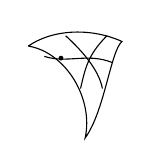
\begin{tikzpicture}[scale=.73]
\draw (0,1.6) .. controls (.46,1.91) and (1.12,1.91) .. (1.63,1.68)
 .. controls (1.43,1.50) and (1.33,.47) .. (.99,0)
 .. controls (1.14,.68) and (.66,1.49) .. (0,1.6);
\draw (.28,1.42) .. controls (.69,1.29) and (1.03,1.49) .. (1.47,1.31);
\draw (.65,1.78) .. controls (.88,1.57) and (1.23,1.21) .. (1.29,.86);
\draw (1.37,1.78) .. controls (1.03,1.44) and (.99,1.20) .. (.91,.86);
\fill (.57,1.39) circle (.042);
\end{tikzpicture}}

% A large X crosses the central working and continues into the Hom calculation below.
\[
\begin{aligned}
&\deleted{(u+v+w)^2=\unsure{u^2}+v^2\unsure{+}w^2+2(uv+vw+wu)}\\
&\deleted{\phantom{(u+v+w)^2}=3+6\cos3\theta=3(1+2\cos3\theta)}
\end{aligned}
\]

\[
\deleted{\left\{\begin{aligned}u+v+w&=\sqrt{3(1+2\cos3\theta)}\,a\\uv&=\cos\theta\\vw&=\cos\theta\\wu&=\cos\theta\end{aligned}\right.}
\]

\[
\begin{aligned}
\cos3\theta&=\cos\theta\cos2\theta-\sin\theta\sin2\theta\\
&=\cos\theta(\cos^2\theta-\sin^2\theta)\\
&\qquad-2\sin^2\theta\cos\theta\\
&=\cos^3\theta-3\sin^2\theta\cos\theta\ \deleted{\unsure{(=\cos\theta-4\mathrm{si}}}\\
&\deleted{=\cos\theta-4\sin^2\theta\cos\theta}\\
&\deleted{3+6\cos3\theta=3+6\cos^3\theta}\\
&\deleted{3+6\cos\theta-24\sin^2\theta\cos\theta}\\
&\cos\theta(1-\underbrace{4\sin^2\theta}_{\deleted{\unsure{\sin^22\theta}}})\\
&\deleted{\unsure{\cos\theta(1-2\sin^2\theta)}}
\end{aligned}
\]

$X\times Y$

\diagram{\begin{tikzcd}[ampersand replacement=\&,column sep=large]
O_X\arrow[r,"{U\mapsto(U,Y)}"]\&O_X\times O_Y\arrow[r,"{(U,V)\mapsto U\times V}"']\&\underline O_{X\times Y}\\
O_Y\arrow[r,"{V\mapsto(X,V)}"']\&{}\&
\end{tikzcd}}

\margin{$\mathrm{Hom}'$: \deleted{\unsure{u}}\inserted{croiss.} commutant aux Sup, quelcon. et Inf finis ;}

\[
\deleted{\operatorname{Hom}'(\underline O_{X\times Y},O)\xrightarrow{u\longmapsto\alpha,\beta}\operatorname{Hom}'(O_X,O)\times\operatorname{Hom}'(O_Y,O)}
\]

\margin{$O$ muni \deleted{Sup} et Inf quelcon, et Inf distributif pour Sup quel}

\deleted{injectif car $u\in\operatorname{Hom}'(O_{X\times Y},O)$ est connu si on connaît ses $u(U\times V)$\inserted{$=\alpha(U)\cap\beta(V)$}, puisque \uline{tout} $W\in O_{X\times Y}$ est Sup de tels $U\times V$.}

Est-ce bijectif ? soit $\alpha:O_X\longrightarrow O$, $\beta:O_Y\longrightarrow O$
Construisons $\gamma:O_{X\times Y}\mathbin{\unsure{-|\to}}O$

posons

\[
\gamma(W)=\operatorname*{Sup}_{\substack{U\in O_X\\V\in O_Y\\U\times V\subset W}}\alpha(\unsure{U|X})\cap\beta(V)
\]

\margin{SPG $\begin{gathered}X\ne\varnothing\\Y\ne\varnothing\end{gathered}$}

C'est une application \uline{croissante} $O_{X\times Y}\longrightarrow O$

\margin{$X'\in\mathrm{Ouv}(X)$}

$\alpha(X'\times Y)=\ ?$ noter que si $Y\ne\varnothing$, alors $U\times V\subset X'\times Y'$ sss $U\subset X'$
donc le Sup est $\deleted{\unsure{\mathrm{Sup}|\text{égal}}}\alpha(X')\cap\beta(Y)=\alpha(X')$
% archive sheet number: 28

\scanpage{31}
\uline{Lemme} $\unsure{\mathscr T|\mathscr E}$ un topos \inserted{loc.} annelé

$C$ Catégorie des couples \unsure{$E\sqrt{\vphantom G G}$|$E,G$} de modules loc. libres de t.f. \inserted{partout $\ne0$}

\margin{(tous les isos)}

$C'$ \rule{3em}{.35pt} quadruples $A,E,F,\varphi$,

\[
\left\{\begin{aligned}
&A\ \text{Algèbre sur }\mathscr T\ \text{loc. isom. à une }\inserted{\text{Alg. de matrices}}\\
&E,F\ \text{Mod. loc. lib. de t.f.}\ \inserted{A,E,F\ \text{partout }\ne0}\\
&\varphi\ \text{un isom. } A\otimes\underline{\mathrm{End}}\,E\simeq\underline{\mathrm{End}}(F).\\
&\hspace{1em}(\text{tous les isos})
\end{aligned}\right.
\]

$F:C\longrightarrow C'$ le foncteur

\[
F:(G,E)\longmapsto\underline{\mathrm{End}}(G),E,G\otimes E,\varphi_{G,E}
\]

où $\varphi_{E,G}$ est l'isom. \uline{can.} $\underline{\mathrm{End}}(G)\otimes\underline{\mathrm{End}}(E)\simeq\underline{\mathrm{End}}(G\otimes E)$

Alors $F$ est une équivalence

\uline{Dém} $F$ provient d'un hom de champs $\underline C\mathbin{\unsure{-|\to}}\underline C'$, et il suffit
de prouver que celui-ci est une équivalence. Or, si $\unsure{g,e|g,f|\mathcal G,\mathcal E}$ sont
deux entiers $\unsure{>|\geq}0$ \inserted{(resp. $a,e,f$ trois entiers $\geq0$)}, soit $\underline C_{g,e}$ le sous-champ de $\underline C$ formé des $E,G$ tels
que rang $E=\unsure{e|g}$, rang $G=g$

(resp. $\underline C'_{a,e,f}$ le sous-champ de $\underline C$ formé des quadruples
pour lesquels $A$ de rg $a^2$, $E$ de rg $e$, $F$ de rg $\unsure{af|f|ae}$)

On a

\[
\underline C_{\deleted{\unsure{g}}}\simeq\coprod_{g,e}\underline C_{\unsure{g}e}\qquad
\underline C'\simeq\coprod_{a,e,f}\underline C'_{a^{\unsure{2}},e,f}
\]

(\uline{somme de champs}) et $\underline F$ induit

\[
\deleted{\unsure{F_{g,e}}}\underline F_{g,e}:\underline C_{g,e}\longrightarrow\underline C'_{g^{2},e,}
\]

on est donc ramené à prouver que les $\underline F_{g,e}$ sont des équivalences.

\uline{Notons} $\underline C_{g,e}$ est une \uline{gerbe} \inserted{trivialisée \deleted{\unsure{liée}} par $\deleted{\unsure{M(\mathcal O_{\mathscr T})}},\ \xi=(\underline O_{\mathscr T}^{g},\underline O_{\mathscr T}^{\unsure{e}}\deleted{\unsure{G}})$} liée par $\underline{\mathrm{GL}}(e)\times\underline{\mathrm{GL}}(g)\simeq\underline{\mathrm{Aut}}(\xi)$

\deleted{$\unsure{\underline C_{g,e}}$} $\underline C'_{g,e}$ est une \uline{gerbe} \deleted{(\unsure{liée par} $\underline{\mathrm{GL}}(e)\times\underline{\mathrm{GL}}(g)$ ?)}
\inserted{(trivialisée par $\xi'=\varphi(\xi)$, \deleted{$\unsure{\mathrm{End}(O_{\mathscr T}^{g}),O_{\mathscr T}^{e},O_{\mathscr T}^{g}\otimes O_{\mathscr T}^{e},\varphi}$}}

\deleted{En effet, $\unsure{\underline C'_{g,e}|\underline C_{g,e}}$ loc (\unsure{et m\textsuperscript{me} globalmt}) a une section}

En effet, \unsure{l'est|c'est} un champ en groupoïdes, \deleted{donc} reste à prouver que
deux objets sont loc. isom. On peut supposer $A=A'$, $E=E'$, $F=F'$,
On considère deux isom $\varphi,\varphi':A\otimes\underline{\mathrm{End}}(E)\rightrightarrows\underline{\mathrm{End}}(F)$
Ils diffèrent par un autom. \deleted{\unsure{intérieur}} de $\underline{\mathrm{End}}(F)$, \deleted{d'où} or tt autom
de $F$ est (localement) intérieur, donc on gagne. \deleted{De plus,}

Pour terminer la démonstration, il reste à prouver
que $\underline F_{g,e}$ induit $\underline{\mathrm{Aut}}(\xi)\xrightarrow{\alpha}\underline{\mathrm{Aut}}(\varphi(\xi))$ qui est un isom.

Or $\xi=(G,E)$ $\xi'=\underline{\mathrm{End}}(G),E,G\otimes E,\varphi_{G,E}:\underline{\mathrm{End}}(G)\otimes\underline{\mathrm{End}}(E)\simeq\underline{\mathrm{End}}(G\otimes E)$

Or si $u,v$ est un autom de $\xi$, $F(u,v)$ est l'aut
$\mathrm{End}(u),v,u\otimes v$, donc si $F(u,v)$ est connu, $v$ est connu et
$u\otimes v$ est connu, d'où \unsure{facilmt|facilemt} (comme $E$ partout non nul) $u$ connu,
donc $\alpha$ injectif. Soit maintenant $\sigma=(\lambda,v,w)$ un autom
% archive sheet number: 30

\scanpage{32}
\diagram{\begin{tikzcd}[ampersand replacement=\&]
C^1\arrow[r]\&C^2\arrow[r]\&C^3\arrow[r]\&C^4
\end{tikzcd}}

\diagram{\begin{tikzcd}[ampersand replacement=\&]
C^1\times Z^2\arrow[d,shift right]\arrow[d,shift left,dash]\&{}\\
\unsure{-\,.\,/}\&-
\end{tikzcd}}

\[
C=\underline{\operatorname{Hom}}(K,K')
\]

\[
\mathrm{TORS}_{\unsure{U|\mathscr U}}^{1}(X,\Pi)\mathrel{\unsure{\overset{\sim}{\to}|\simeq}}\mathbb H^1(X,\Pi)
\]

% Long diagonal strokes run across the ruled sheet.
\diagram{\begin{tikzcd}[ampersand replacement=\&,column sep=small,row sep=small,
execute at end picture={\draw ([xshift=-4pt,yshift=5pt]\tikzcdmatrixname-1-3.north west) rectangle ([xshift=4pt,yshift=-3pt]\tikzcdmatrixname-2-3.south east);
\draw ([xshift=-3pt]\tikzcdmatrixname-1-2.north west) rectangle ([xshift=3pt]\tikzcdmatrixname-1-2.south east);
\draw (\tikzcdmatrixname-1-3.north west) to[bend right=12] (\tikzcdmatrixname-1-3.north) to[bend right=12] (\tikzcdmatrixname-1-3.north east);
\draw (\tikzcdmatrixname-3-3.south west) -- (\tikzcdmatrixname-3-4.south east);}]
\mathrm{Hom}\unsure{(\,.\ .|.\ .}={}\&|[draw,circle,inner sep=1pt]|C^0\arrow[r,leftrightarrow]\&C^0\times Z^1\arrow[d,shift left]\arrow[d,shift right]\&{}\\
{}\&{}\&|[draw,circle,inner sep=1pt]|\underline{Z^1}\arrow[r,leftrightarrow]\&\overset{\mathbb H^2}{C^1\times Z^2}\arrow[d,shift left]\arrow[d,shift right]\&{}\\
{}\&{}\&|[draw,rounded corners]|\operatorname{Aut}(0)\&0=\underline Z^2\arrow[r,leftrightarrow]\&{}
\end{tikzcd}}

\diagram{\begin{tikzcd}[ampersand replacement=\&]
0\arrow[r,shift left]\arrow[r,shift right]\arrow[r,phantom,"\unsure{\downarrow}"]\&0
\end{tikzcd}}

\diagram{\begin{tikzcd}[ampersand replacement=\&]
{}\&K\arrow[dl]\arrow[d,shift right]\arrow[d,shift left]\\
K'\&K'\arrow[u,shift left=2]
\end{tikzcd}}

\[
 f-f'=dk\mathbin{\unsure{-|+}}kd\qquad \deleted{\unsure{kd-dk}}
\]

\diagram{\begin{tikzcd}[ampersand replacement=\&]
T^n=\text{\uuline{$\mathrm{TORS}^{n}_{U}(X,\Pi)$}}
\arrow[r,shift right=1.3,"\unsure{2|Z}"']\&
|[draw,rounded corners]|{\mathbb H^n(X,\Pi)}
\arrow[l,bend right=20,"\unsure{Z|2}"']\&
{\Rightarrow\ \pi_0(T^n)\xrightarrow{\sim}H^n(X,\Pi)}
\end{tikzcd}}

\[
\mathrm{TOR}^{1}_{\unsure{\mathscr T|\tau|U}}(X,\Pi)\xrightarrow{\approx}\mathbb H^1(X,\Pi)
\]

\diagram{\begin{tikzcd}[ampersand replacement=\&,row sep=small,execute at end picture={\draw ([xshift=-50pt]\tikzcdmatrixname-4-1.north west) to[bend left=3] ([xshift=90pt]\tikzcdmatrixname-4-1.north east);}]
E_{\unsure{2|\bullet}}\arrow[d]\arrow[d,shift right=1.5]\arrow[d,shift left=1.5]\&{}\\
E_1\arrow[d,shift right]\arrow[d,shift left]\&{}\\
E_0\arrow[d]\&1\\
X\&{}
\end{tikzcd}}

\diagram{\begin{tikzcd}[ampersand replacement=\&,row sep=small]
\deleted{X\times\Pi}\&\Pi\arrow[d,dash]\\
\Pi\times E\arrow[d,shift left]\arrow[d,shift right]\&1\\
E\arrow[u,bend left=42,dashed]\arrow[d]\&{}\\
X\arrow[u,bend left=42,dashed]\&\unsure{\infty/1}
\end{tikzcd}}
% archive sheet number: 31

\scanpage{33}
de $\xi'$, donc

\[
\left\{\begin{aligned}
&\lambda\ \text{un autom de }\underline{\mathrm{End}}(G),\\
&v\qquad\rule{2.8em}{.35pt}\qquad E\\
&w\qquad\rule{3em}{.35pt}\qquad G\otimes E
\end{aligned}\right.
\]

avec commutativité de

\diagram{\begin{tikzcd}[ampersand replacement=\&]
\underline{\mathrm{End}}(G)\otimes\underline{\mathrm{End}}(E)
 \arrow[r,"\varphi_{G,E}","\sim"']\arrow[d,"\lambda\otimes\mathrm{End}(v)"']
 \&\underline{\mathrm{End}}(G\otimes E)\arrow[d,"\mathrm{End}(w)"]\\
\underline{\mathrm{End}}(G)\otimes\underline{\mathrm{End}}(E)
 \arrow[r,"\varphi_{G,E}"]
 \&\underline{\mathrm{End}}(G\otimes E)
\end{tikzcd}}

\deleted{On sait} Il suffit de voir que \uline{loc} il provient d'un \deleted{$(u,v)$}
autom de $\xi$, qui sera de la forme $(u,v)$, $u$ un autom
de $G$, donc on veut prouver

\[
\lambda\simeq\mathrm{End}(u),\quad w=u\otimes v
\]

Or on sait que loc. $\lambda$ est \deleted{\unsure{induit}} intérieur, i.e. \unsure{que|qu'|qu'il} \inserted{loc}
\unsure{on} peut trouver $u$ tel $\lambda=\mathrm{End}(u)$. Quitte à multiplier \inserted{$\sigma$} par
$F(u,v)^{-1}$, on peut supposer que $\lambda=\mathrm{id}$. Donc on \deleted{est} a
$\varphi\circ(\mathrm{id}\otimes\mathrm{End}(v))\simeq\mathrm{End}(w)\circ\varphi$, et on doit prouver qu'il existe [loc.]
une section $u$ de $\underline O_{\unsure{T|\mathscr T}}^{*}$ telle que $w=\unsure{u}( \mathrm{id}_{G}\otimes v)$, \deleted{\unsure{or}} \inserted{i.e. $w=\mathrm{id}_{G}\otimes uv$}

\deleted{prenant la sous-algèbre $1_G\otimes\underline{\mathrm{End}}(E)$ de $\underline{\mathrm{End}}(G)\otimes\underline{\mathrm{End}}(\unsure{G|E})$
la commutativité \deleted{\unsure{postule|postulée|partielle}} donne}

\[
\begin{aligned}
&\deleted{\mathrm{End}(w)(\mathrm{id}_G\otimes X)=\mathrm{id}_G\otimes\mathrm{End}(v)(X)\qquad \text{pour }X\in\Gamma\,\mathrm{End}(E)}\\
&\deleted{w(\mathrm{id}_G\otimes X)w^{-1}=\mathrm{id}_G\otimes vXv^{-1}}
\end{aligned}
\]

L'hyp. de compatibilité
s'écrit que pour tt end. $X$ de $G$, $Y$ de $E$, on a

\[
\deleted{\unsure{\varphi(X\otimes Y)}}\quad
w\circ(\underbrace{X\otimes Y}_{\substack{\text{endom}\\\text{produit}\\\text{tensoriel}\\\text{de }G\ \mathrm{et}\ E}})w^{-1}
=\underbrace{X\otimes{}}_{\mathrm{id}}vYv^{-1}
\]

donc $\mathrm{End}(w)$ est un autom. \inserted{connu} de $\mathrm{End}(G\otimes E)$ \inserted{$\simeq\underline{\mathrm{End}}(G)\otimes\underline{\mathrm{End}}(E)$}
\deleted{qui \unsure{commute} à l'action de $\mathrm{End}(G)$, donc elle est déterminée par
son action sur $1_G\otimes\mathrm{End}(E)$ \unsure{donnée}} savoir il
est égal à la troisième composante de $\deleted{F(\mathrm{id}_G,v)}\inserted{\mathrm{End}(\mathrm{id}_G\otimes v)}$, \deleted{Donc}
\deleted{$w$} Donc $w$ en diffère par une \deleted{unité} section, cqfd.

\uline{Corollaire} \deleted{Le lemme reste valable si on remplace $C'$ par la catégorie \unsure{des quadruples} tels}
\inserted{Soit $A$ une Algèbre \deleted{d'Azumaya} sur $\mathscr T$}
\deleted{[loc libre de t.f. \unsure{rg|sg} partout non nulle, $A^{o}\otimes A\xrightarrow{\sim}\underline{\mathrm{End}}(A)$]}
telle qu'il existe $E,F$ modules loc. libres de t.f. \deleted{tel que}\inserted{et un isom}
$A\otimes\underline{\mathrm{End}}(E)\xrightarrow[\sim]{\varphi}\underline{\mathrm{End}}(F)$ \inserted{donné}
Alors \deleted{$A$ est loc} $\exists G$ loc libre de t.f. [partout non nul]
\deleted{tel que}\inserted{et} $A\xrightarrow[\sim]{\psi}\mathrm{End}(G)$, de plus $G,\psi$ est déterminé
à isom unique près.

En effet, l'hyp implique que $A$ est loc libre de t.f. comme
Module, de plus $A^o\otimes A\otimes\mathrm{End}(E)\simeq A^o\otimes\mathrm{End}(F)$
% archive sheet number: 32

\scanpage{35}
Recall: direct and inverse images
\inserted{+ \uline{examples}} fiber functor as inverse image / case of an \unsure{etale|étale} morphism:
its base change \uline{inside} $\operatorname{Top}(X)$.
direct img of \inserted{sheaves with} algebraic structures versus inverse img
\inserted{(defined by \unsure{$\underline{\mathrm{Lim}}$|$\underline{\mathrm{Hom}}$})}
(defined by finite $\varprojlim$ \uline{and} by \uline{$\lim$})

% slanted
\margin{sheaf of ordered sets}

\margin{Constant sheaves \deleted{Sheaves} $\underline{\mathrm{Hom}}(F,G)$ and $\unsure{\Gamma|p|\beta}(F)$. Their intrinsic caracter. $\Gamma(F)\simeq\underline{\mathrm{Hom}}(F,\unsure{p^{-1}(e_1)|\beta(e_1)})$. $\operatorname{Top}(X)\simeq$ functors $\operatorname{Top}(X)^o\to(\mathrm{Ens})$ which commute with $\varprojlim$}

\uline{Examples}: field, integral domain.
\deleted{\unsure{Ex}}Example: product of epimorphisms not an epimorphism.

\uline{``The abstract category $T(X)$ embodies all topological information worthwhile for $X$'':}

a) \deleted{sheaves with} \inserted{the notion of} alg. structures on $X$ can be reconstructed from $T(X)$

b) The notion of \uline{stack} over $X$ depends on $T(X)$ \deleted{alone}\inserted{alone}
(up to equivalence)

c) connexity of $X$, \deleted{\unsure{commutative H}} cohomology and homotopy
invariants (cf SGA4 $\underline{\mathrm V}$ and Artin \& Mazur)

d) Relation between $\pi_1$ and covering spaces of $X$

\unsure{e)} Non commutative hom algebra: $\unsure{H^1|H^i}(\ ,\ )$

f) Other examples: local connectedness; total disconnectedness
\unsure{quasi}-compactness ---

g) Operations on spaces (sums, amalgamated sums \inserted{---})
and properties of \inserted{their} continuous maps reflected
by operations on topoi.

\uline{The ``reasonable'' spaces $X$ can be recovered from $\operatorname{Top}(X)$, and so can the continuous maps.}

\margin{\uline{NB} $\uline{\mathrm{Fib}}(E)$ is \uline{rigid} if $E=\operatorname{Top}(X)$}

$\operatorname{Fib}(E)$ (isomorphism classes of \inserted{generalized} fiber functors) as a
topo space. It corresponds to the set $\bar X$ of
all closed irreduc. subsets of $X$, with the
obvious topology, and

\deleted{$\unsure{X\to\mathrm{Fib}(E)}$}

$X\mathbin{\unsure{-|\to}}\operatorname{Fib}(E)$ can be identified with $x\longmapsto\overline{\{x\}}$
The topology of $X$ is the inverse image topology.

% slanted
\margin{\unsure{Start with|Start with the} defining and studying $\bar X$, $i:X\to\bar X$ and the fact that it induces $i^*:\mathscr O_{\bar X}\xrightarrow{\sim}\mathscr O_X$ and hence \deleted{\unsure{equiv.}} isomorphisms $i^*:\operatorname{Top}(X)\xleftarrow{\sim}\operatorname{Top}(\bar X)$ and hence also $i_*:\operatorname{Top}(\widetilde X)\mathrel{\unsure{\simeq|\xrightarrow{\sim}}}\operatorname{Top}(X)$, \unsure{equivalence}, $i_*=i^{*-1}$. \unsure{if we choose this, we are evident|if we choose this more evident} \unsure{we have} a map $\bar X\to\operatorname{Fib}(\operatorname{Top}(X))$. That \deleted{\unsure{it is bij.}} it is injective is clear, that it is bijective is a little more subtle -- it is done as \deleted{\unsure{the}} exercise in SGA4, or in \unsure{Mme.|other} \unsure{Hakim's} book ....}

map injective $\Longleftrightarrow\ \bar x=\bar y\ \Rightarrow x=y$ (i.e. sep\textsuperscript{n} axiom that $x\ne y$ implies
that either $x$ or $y$ has a neighbourhood not containing the other)

\deleted{\unsure{inj.}} surjective $\Longleftrightarrow$ every closed irreduc. subset of $X$ has a generic pt.

\deleted{so-called} map bijective $\Longleftrightarrow$ $x\mapsto\bar x$ is a bijective map \deleted{from} $\widetilde X$:

\[
X\quad\text{\uline{sober}}
\]

[$X\longrightarrow\widetilde X$ can be viewed as being the universal map of $X$
into a sober space, $X\longmapsto\widetilde X$ the left adjoint of
the inclusion $(\unsure{\mathrm{Esp}|\mathrm{Sp}}\ \mathrm{sob})\longrightarrow(\mathrm{Esp})$

\[
\operatorname{Hom}_{\mathrm{Sp\,sob}}(\unsure{X|\widetilde X},i(Z))\simeq\operatorname{Hom}_{\mathrm{Sp}}(\widetilde X,Z)
\]

Thus $X\mapsto\bar X$ commutes with arbitrary $\varinjlim$ ....]

\margin{best case of so-called Jacobson spaces to be considered}

Thus 1) Sober spaces can be reconstructed from their $\operatorname{Top}(X)$
(and they are the only ones, in a certain sense)

Moreover 2) If $X$ arbitrary, then $X\to\widetilde X$ induces $f^*:\operatorname{Top}(\widetilde X)\to\operatorname{Top}(X)$
an equivalence (hence too an equivalence,
% archive sheet number: 34

\scanpage{36}
\mspage{1}
$T$ espèce de structure ``définie par $\varprojlim$ finies'' (resp. quelc.)
sur famille d'ens de base $(E_i)_{i\in I}$ ($I$ ens. donné)

Pour toute catégorie $C$ avec $\varprojlim$ finies (resp. quelconques)
on a donc

\[
T(C)\xrightarrow{\varphi_C^T}C^I
\]

foncteur \inserted{``famille d'objets de $C$ sous-jacente''} allant de la catégorie des ``structures d'espèce
$T$ dans $C$'' vers $C^I$. Pour tt foncteur

\[
u:C\mathbin{\unsure{-|\to}}C'
\]

commutant aux $\varprojlim$ finies (resp. quelc.) on a de plus

\[
T(C)\xrightarrow{T(u)}T(C'),
\]

rendant commutatif le diagramme

\diagram{\begin{tikzcd}[ampersand replacement=\&]
T(C)\arrow[r,"T(u)"]\arrow[d,"\varphi_C^T"']\&T(C')\arrow[d,"\varphi_{C'}^T"]\\
C^I\arrow[r,"u^I"']\&C'^I
\end{tikzcd}}

On a $T(\mathrm{id}_C)=\mathrm{id}_{T(C)}$, $T(vu)=T(v)T(u)$, donc $T$ est un
\uline{foncteur} $\unsure{\xi}$ de $\unsure{L_\infty|\mathcal L_\infty|L_0}=(\mathrm{Cat}\ \varprojlim\ \mathrm{finies})$ (resp. $\unsure{L_0|\mathcal L_0}=(\mathrm{Cat}\ \varprojlim)$) dans
$\mathrm{Cat}$, d'où \deleted{\unsure{on a|on}} une catégorie \inserted{co}fibrée \inserted{$T$} sur $\unsure{L_\infty}$ (resp. $L_0$)
munie d'un \deleted{foncteur}\inserted{morphisme de cat} cofibrées de $T$ dans \inserted{la cat. cofibrée} $\unsure{\tau_I|T_I|\mathcal T_I}:C\mathbin{\unsure{-|\to|\mapsto}}C^I$.

\[
\varphi^T:T\longrightarrow \tau_I
\]

\deleted{\unsure{Hom}} Soit $T'$ une autre ``espèce de structure'' \inserted{sur $I'$}, Alors on définit

\[
\begin{aligned}
\underline{\mathrm{Hom}}_{\unsure{4|\xi|L}}(T,T')&=\underline{\mathrm{Hom}}_{L_\infty}(T_{L_\infty},T'_{L_\infty})\\
{}[\text{resp }\underline{\mathrm{Hom}}_{4}(T,T')&=\underline{\mathrm{Hom}}_{L_0}(T_{L_0},T'_{L_0})]
\end{aligned}
\]

et si $I=I'$

\[
\begin{aligned}
\underline{\mathrm{Hom}}_{4}(I;T,T')={}&\text{catégorie des hom de }T_{L_\infty}\text{ dans }T'_{L_\infty}\\
&\text{munis d'un isom de compatibilité}
\end{aligned}
\]

\diagram{\begin{tikzcd}[ampersand replacement=\&]
\alpha:\quad T_{L_\infty}\arrow[rr,"u"]\arrow[dr,"\varphi^T"']\arrow[rr,phantom,shift right=2.5,"\overset{\sim}{\longrightarrow}_{\alpha}"']\&{}\&T'_{L_\infty}\arrow[dl,"\varphi^{T'}"]\\
{}\&\deleted{\unsure{(\tau_I)_{L_0}}}(\tau_I)\&{}
\end{tikzcd}}

[resp. $\underline{\mathrm{Hom}}(I;T,T')=$ \hspace{2em}]
% A long oblique stroke runs from the first limit to the line beginning ``Soit T'''.
% archive sheet number: 35

\scanpage{37}
in other words $X$ and $\bar X$ have the same sheaf theory:
For all \inserted{(most?)} practical purposes, $X$ can be replaced with $\widetilde X$.

\deleted{\unsure{it}} We have a map

\[
\operatorname{Hom}_{\mathrm{Sp}}^{\unsure{\prime\prime}}(X,Y)\longrightarrow
\operatorname{Hom}_{\mathrm{top}}(\operatorname{Top}(X),\operatorname{Top}(Y))
\qquad(\text{isom classes})
\]

it is bijective if $Y$ is sober. In fact, the category $\underline{\mathrm{Hom}}_{\mathrm{top}}(\operatorname{Top}(X),\operatorname{Top}(Y))$
is \deleted{discrete}\inserted{rigid}, associated to an order relation on $\operatorname{Hom}_{\mathrm{top}}(\operatorname{Top}(X),\operatorname{Top}(Y))$
(specialisation) !

\uline{The notion of a topos}. \inserted{(gener\unsure{.?|al.?|.}) ``topology'' $=$ study of topoi,}
Why it is a natural and useful generalisation of the notion of topological space?

a) It is the natural setting for most ``algebraic'' (and non algebraic) structures.

b) As such, it allows to construct classifying topoi for such structures (possibly all): algebra = topology !

c) It is stable under a variety of operations that in many cases do not make sense in the category of topological spaces:
$*$ generalized notions of passage to quotient (by wild equivalence relations, which would give pathological quotients within top. spaces)

$*$ clutching together of pieces à la Artin

d) They arise in various questions \inserted{of geometry} as modular topoi

e) They provide the most convenient set-up for
\inserted{all topics involving systematically} \deleted{\unsure{this}} passing to quotients.

f) They give the ultimate outcome for \inserted{the intuitive notion of} localization.

g) They are technical musts for various cohomology theories
in algebraic geometry.

\uline{Examples of topoi}

\[
\left\{\begin{aligned}
&\operatorname{Top}(X),\quad \operatorname{Top}(X,G)
 \left\{\begin{aligned}&\operatorname{Top}(\unsure{X|X'})\\&B_G\quad H^{\unsure{q|*}}(G,-)\end{aligned}\right.\\
&\widehat C\quad\text{for instance }B_G\ (G\text{ discrete})
\end{aligned}\right.
\]
% archive sheet number: 36

\scanpage{38}
\mspage{3}
Si $T$ est donné avec $I$, on a une application canonique

\[
 I\longrightarrow\mathrm{Ob}\,\Gamma^{T}_{\unsure{*|\xi|\varphi}}
 \qquad(\text{resp. }I\mathbin{\unsure{-|\to}}\mathrm{Ob}\,\Gamma_{\unsure{0|\varphi|\varphi_0}}^{T})
\]

On a, si $T$ est \unsure{via|de} $\varprojlim_{\unsure{\bullet|0}}$, un foncteur

\[
\Gamma^{T}\longrightarrow\Gamma_0^{T}
\]

(Cas particulier de \hspace{1em} pour $T'=\tau$) et on a
commutativité dans

\diagram{\begin{tikzcd}[ampersand replacement=\&]
\mathrm{Ob}\,\Gamma^T\arrow[rr]\&{}\&\mathrm{Ob}\,\Gamma_0^T\\
{}\&I\arrow[ul]\arrow[ur]\&{}
\end{tikzcd}}

\deleted{\unsure{Ex Supposons}}
\uline{\unsure{Ex|Exp|Ex.}} Supposons qu'il existe une $\beta^{T}_{*}\in(\mathrm{Cat}\ \varprojlim_{\bullet})$
(resp. $\beta^{T}_0\in(\mathrm{Cat}\deleted{\unsure{*}}\varprojlim)$) telle que $T$ (resp. $T_0$)
soit \deleted{\unsure{déf|défini}} 2-représenté par \unsure{cet} objet:

\[
\begin{aligned}
T(C)_{\unsure{*|\bullet}}\mathrel{\mathop{=}^{\approx}}\underline{\mathrm{Hom}}_{\varprojlim_{\bullet}}(\beta^{\unsure{*|T}},C)
&\qquad C\in\mathrm{Ob}(\mathrm{Cat}\ \varprojlim_{\bullet})\\
(\quad T(C)\mathrel{\mathop{=}^{\approx}}\underline{\mathrm{Hom}}_{\varprojlim}(\beta_0,C)
&\qquad C\in\mathrm{Ob}(\mathrm{Cat}\ \varprojlim)
\end{aligned}
\]

Alors a) $\beta$ $(\beta_0)$ est défini à équivalence près,
\deleted{\unsure{définie à|défini}} unique à isom unique près

b) Pour tte catégorie $\unsure{2'|2}$-cofibrée $\mathcal F$ \inserted{$(\mathcal F_0)$} sur $(\mathrm{Cat}\ \varprojlim_{\bullet})$
(resp. $(\mathrm{Cat}\ \varprojlim)$) on a, équiv. can.

\[
\begin{aligned}
\underline{\mathrm{Hom}}(T,\mathcal F)&\mathrel{\mathop{=}^{\approx}}\mathcal F(\beta_{\unsure{*}})\\
(\underline{\mathrm{Hom}}_0(T,\mathcal F)&\mathrel{\mathop{=}^{\approx}}\mathcal F(\beta_0))
\end{aligned}
\]

en particulier, si $\mathcal F$ est défini par $\unsure{T|T'}$ on aura

\[
\begin{aligned}
\underline{\mathrm{Hom}}(T,T')&\mathrel{\mathop{=}^{\approx}}T'(\beta)\\
(\underline{\mathrm{Hom}}_0(T,T')&\mathrel{\mathop{=}^{\approx}}T'(\beta_0))
\end{aligned}
\]

et en particulier, faisant $T'=\unsure{\iota|i}$, \deleted{\unsure{resp|struct}} on a $T'(\beta)=\beta$ $(T'(\beta_0)=\beta_0)$
on trouve

\[
\begin{aligned}
\beta&=\underline{\mathrm{Hom}}(T,\iota)=\Gamma^{T}\\
(\beta_0&=\underline{\mathrm{Hom}}_0(T,\iota_0)=\Gamma_0^{T})
\end{aligned}
\]
% A long oblique stroke traverses the hypothesis and its consequences.
% archive sheet number: 37

\scanpage{39}
Compléments on relations between $X$ and $\operatorname{Top}(X)$

a) Specialisation and morphisms between fiber functors

If $x\in\overline{\{y\}}$, then We have a functorial homomorphism
$F_x\mathbin{\unsure{-|\to}}F_y$ ($F\in\mathrm{Ob}\,\operatorname{Top}(X)$) because the neighbourhoods of
$y$ contain $x$. Thus \deleted{\unsure{this}} we get \deleted{\unsure{that}}

\[
\mathrm{Cat}(X\ \text{ordered by }x\leq y\ \text{iff }x\in\overline{\{y\}})\longrightarrow
\underline{\mathrm{Fib}}(\operatorname{Top}(X))
\]

\uline{Proposition} $\mathrm{Hom}(E_x,E_y)=\left\{\begin{array}{ll}\varnothing&\text{if }x\nleq y\quad\text{i.e.}\\\text{reduced to the specialisation hom otherwise}\end{array}\right.$
i.e. the previous functor is fully faithful

\uline{Corollary} If $X$ sober \deleted{(and only then)} \inserted{more generally if $X\to\bar X$ surjective} (i.e. ---)
then (and only then ... !) the previous functor is an equivalence.

% slanted
\margin{\uline{NB} in the case of Hausdorff (or $T_1$ spaces where pts are closed) spaces, we get a discrete category of fiber functors.}

b) ($\mathrm{Cat}\ \unsure{\mathrm{Hom}|\mathrm{hom}|\underline{\mathrm{Hom}}}(X,Y)$ ordered by $f\leq g$ iff $\forall x\in X,\ f(x)\in\overline{\{g(x)\}}$).
\inserted{Assume $X$, \deleted{\unsure{sober}} \inserted{for simplicity} \deleted{\unsure{and}}}

\diagram{\begin{tikzcd}[ampersand replacement=\&]
{}\arrow[d]\\ \underline{\mathrm{Hom}}(\operatorname{Top}(Y),\operatorname{Top}(X))
\end{tikzcd}}

% slanted
\margin{\unsure{Voilà|No !} \unsure{l'explication|il s'agit} \unsure{pour la recherche|pour redresser} \unsure{d'une notion|une notion} \unsure{d'espace|ancienne} \unsure{propre via topos|propre bien topol|certain topoi}.}

% slanted
\margin{if $Y$ is reduced to a point, we get back}

\uline{fully faithful} \deleted{\unsure{if $X$ is sober}}
its essential image consists of the $f^{*}$'s that are
left exact and commute with $\varinjlim$. \deleted{and
it's the whole of it whenever $Y$ is}

\uline{Topos.}

\uline{1)} \uline{Definition} a) Through exactness properties + generators
for \unsure{example|examp.|instance} \inserted{Giraud's} a) b) c) d)

\deleted{\unsure{b)|$*$}} Many sets of equivalent exactness properties possible.
What will insure that a given set will \deleted{satisfy}\inserted{imply}
whatever other property .... comes up ?

The original definition was \deleted{in fact} in terms of
categories of (generalized sheaves \inserted{$=$ \unsure{foncteurs|faisceaux} \unsure{particuliers|ponctuels}}) on categories generalizing \deleted{\unsure{open}} the categories \deleted{\unsure{Cat}} $O_X$. We cannot
express it now, but we can express

\diagram{\begin{tikzcd}[ampersand replacement=\&]
\text{b)}\quad E\arrow[r,"{\text{fully faithful}}","f_*"']\&\text{some }\widehat C\\
{}\& C\ \text{``small''}
\end{tikzcd}}

with a left adjoint $f^*$ which is \uline{left exact}.
% archive sheet number: 38

\scanpage{40}
Considérons l'espèce de structure ``anneau (comm. unifère)'', soit $T$.
On sait qu'elle est définie en termes de produits finis
soit $\lambda_0$ \inserted{$=(\text{ensembles finis},\varnothing)$} le type de structure correspondant. \deleted{On se propose de \unsure{$\xi$}, étudier}
\inserted{Donc $T$ définit un $\lambda_0$-type $T_{\lambda_0}$,}
donc pour tout $\lambda$ type tel que $\lambda_0\longrightarrow\lambda$ (les
$\lambda$-catégories ont des produits finis, les $\lambda$-foncteurs y commutent)
il définit un $\lambda$-type $T_\lambda$. On se propose, pour divers
$\lambda$, d'étudier l'existence \inserted{et l'unicité} d'un sous-type plein $T_\lambda^*$
($T_\lambda^*(C)\mathbin{\unsure{-|\to}}T_\lambda(C)$ pl. fidèle pour tout $C$) de telle façon que
pour $C=(\mathrm{Ens})$, $T_\lambda^*(C)$ soit la sous-catégorie \inserted{str.} pleine de
$T_\lambda(C)$ \inserted{$=(\mathrm{Ann})$} $=$ cat. des anneaux (comm. unifères) qui sont des \uline{corps} \unsure{$\xi$}
(commutatifs). [On sait que l'unicité est acquise si $\lambda=(\underset{\leftarrow}{\lambda}_1,\underset{\longrightarrow}{\lambda}_2=\varnothing)$].

a) Si $\lambda=\lambda_0$, \uline{il n'existe pas} une telle $T_\lambda$. En effet, \deleted{\unsure{en termes}} \deleted{\unsure{$\lambda$ produit}}
si $\lambda=(\underset{\leftarrow}{\lambda}_1,\underset{\rightarrow}{\lambda}_2=\varnothing)$, $\underset{\leftarrow}{\lambda}$ formé de \unsure{diagrammes|diag. non} finis, alors
$T_\lambda$ est $\lambda$-\unsure{représenté|représentable} par la $\lambda$-catégorie \inserted{$\mathcal R_{\lambda}^{T}$} qui est \inserted{l'opposé de} la sous-catégorie pleine $S_\lambda^T$ de Ann engendrée (pour les $\varinjlim$ de type $\unsure{\lambda_1|\lambda_3}$)
par $\mathbb Z[T]$ (l'objet libre engendré par 1 élément). Les sous-\deleted{catégories}types pleins de $T_\lambda$ \deleted{sont les} correspondent aux
catégories de fractions de $\mathcal R_\lambda^T$ par des ens. de flèches $M^*$
stables par composition, et par $\varprojlim$ de type $\lambda_1$ (ou aux
cat. \deleted{\unsure{quot.|quotient}} de fractions à \uline{gauche} pour $S_\lambda^T$ par des ens
$M$ de flèches stables par $\varinjlim$ de type $\lambda_1$). Ici, \deleted{des}\inserted{l'ens $M$}
flèches en question \deleted{\unsure{sont}}\inserted{est} \deleted{celles}\inserted{formé} des flèches $u:A\mathbin{\unsure{-|\to}}B$
dans $S_\lambda^T$ \inserted{$\subset(\mathrm{Ann})$} telles que pour tout \deleted{\unsure{k}} \uline{corps} $k\in\mathrm{Ob}(\mathrm{Ann})$,
la flèche $\mathrm{Hom}_{\mathrm{ann}}(B,k)\longrightarrow\mathrm{Hom}_{\mathrm{ann}}(A,k)$ soit \uline{bijective}, [ou
encore que le \deleted{\unsure{hom}} morphisme de schémas affines $u':X\mathbin{\unsure{-|\leftarrow|\to}}\deleted{Y}$
défini par $u$ soit tel que $X(k)\xrightarrow{\sim}Y(k)$ pour tt corps $k$.
On sait que cela signifie que $u$ est \uline{bijective} et définit
des ext. résiduelles triviales] \deleted{\unsure{Alors}} Cet ens de flèches
est évidemment stable par composition et par $\varinjlim$ (resp. $\varprojlim$)
de type $\lambda_1$ (serait vrai pour tte \unsure{sous|ss}-catégorie de (Ann),
% The ruled sheet is upside down in the scan; long oblique pen stroke through the working.
% archive sheet number: 39
